\section{Architectural Views}

\subsection{Context View}

\subsubsection{Stakeholders' Uses of This View}

\subsubsection{Context Diagram}

% Checked in grammarly
\afetbilgi \cite{afetbilgi} is not part of a more extensive system. It is a standalone and open-source efforted website to verify critical information in the fight against the 6 February 2023 Pazarcik Earthquake and deliver it to disaster victims and those who want to help in an understandable, concise manner in multiple languages.

This information is presented in either the form of legible tables with third-party governmental and private links or an interactable method via a map view interface. If deemed necessary, admin and maintainers can make changes to display newly created or edited data and upload it to the system upon any complaints or suggestions they may get on their contact details.

\begin{figure}[H]
  \centering
  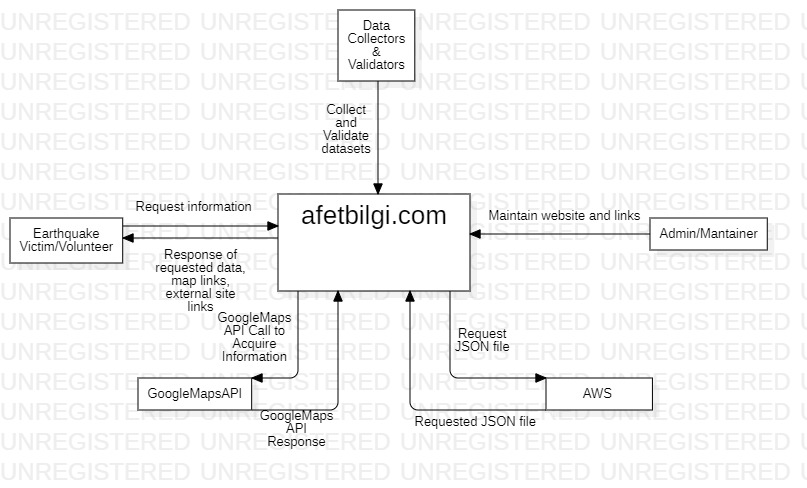
\includegraphics[width=\linewidth]{img/context-diagram.jpg}
  \caption{Context Diagram for \afetbilgi}
\end{figure}

The \afetbilgi\ consists of a combination of small physical and software parts. With the help of interfaces, these parts communicate among themselves and with the user.

\subsubsection{External Interfaces}

In this section, the external interfaces of the \afetbilgi will be provided, as well as their operations and relationships.

\begin{figure}[H]
  \centering
  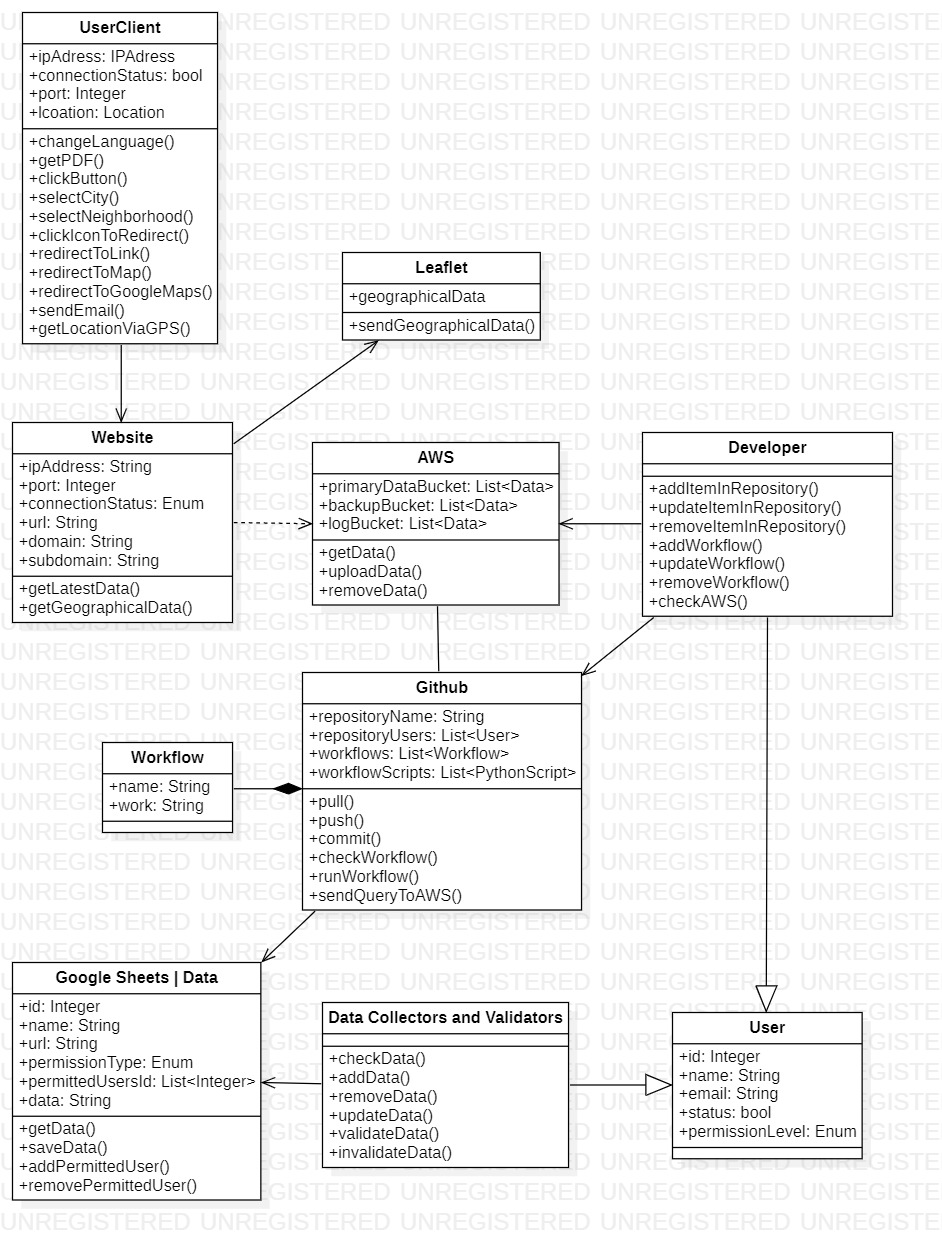
\includegraphics[width=\linewidth]{img/external-interfaces-diagram.jpg}
  \caption{External Interfaces}
\end{figure}

As it can be observed from Figure \addnumbertofigure{0}, \afetbilgi has multiple external interfaces. UserClient, Website, Leafler, AWS, Developer, Google Sheets for data, Data Collectors and Validators are external interfaces of the system. Github Repository for the \afetbilgi may also ve considered an external interface since it is generally responsible for sustainability of the system. The operations given in the diagram can be summarized as follows:

\begin{itemize}
  \item The Data Collectors and Validators collect data and validate it. After validation, data is added into a specificied data sheet in Google Sheets.
  \item Google Sheets mainly store the data. The data is divided into several files in Google Sheets. These sheets can be accessible for data collectors and validators.
  \item GitHub Repository is used storing the source code. Additionally, the GitHub workflows of the repository check, maintain and update the website in regular basis by executing the workflows in a determined period.
  \subitem Some workflows use the scripts in the repository to access sheets to get the recent data and create new updated \texttt{latest.json} and \texttt{schema.json} files. After completing the creation of these files, they are uploaded to Amazon Web Services (AWS). These workflows can be managed and updated by the developer.
  \item Leaflet is used for the map of the afetbilgi. There is additional subdomain, whose link is \href{https://maps.afetbilgi.com}{maps.afetbilgi.com} for the complete map.
  \item UserClient initiate the connection with the website. It has some attributes that are provided to website and functionalities to control the website.
\end{itemize}

\subsubsection{Interaction Scenarios}

Two different interaction scenarios are provided:

\begin{figure}[H]
  \centering
  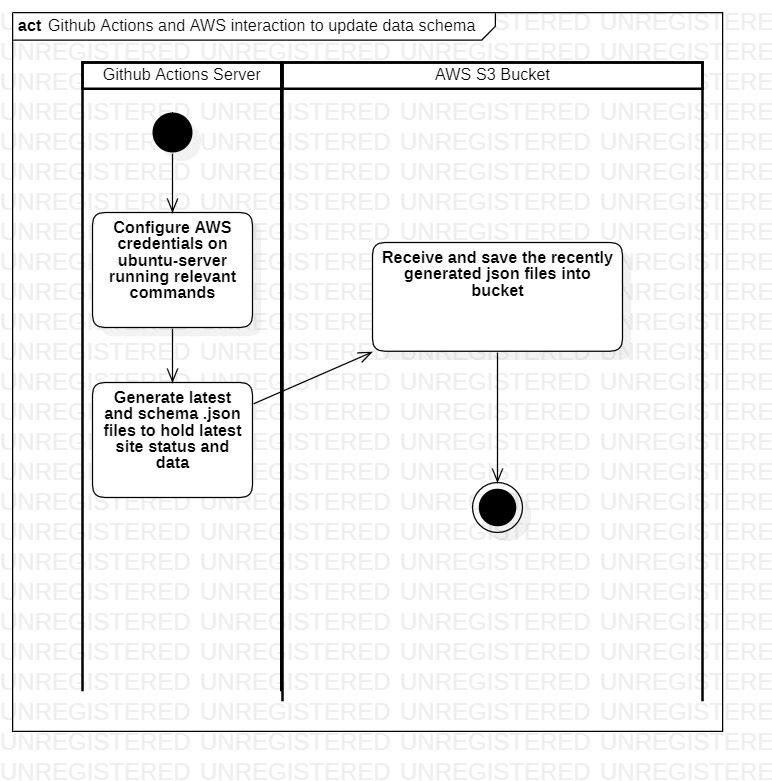
\includegraphics[width=\linewidth]{img/activity-diagram-1.jpg}
  \caption{Activity Diagram | GitHub Actions and AWS Interaction to Update Data Schema}
\end{figure}

\begin{figure}[H]
  \centering
  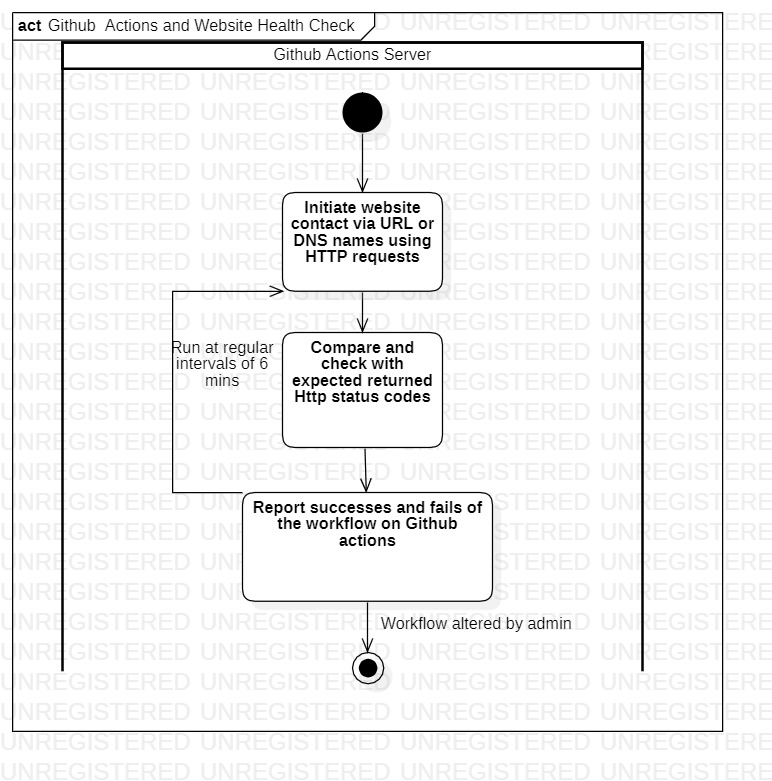
\includegraphics[width=\linewidth]{img/activity-diagram-2.jpg}
  \caption{Activity Diagram | GitHub Actions and Website Health Check}
\end{figure}

\subsection{Functional View}

\subsubsection{Stakeholders' Uses of This View}

\subsubsection{Component Diagram}

\begin{figure}[H]
  \centering
  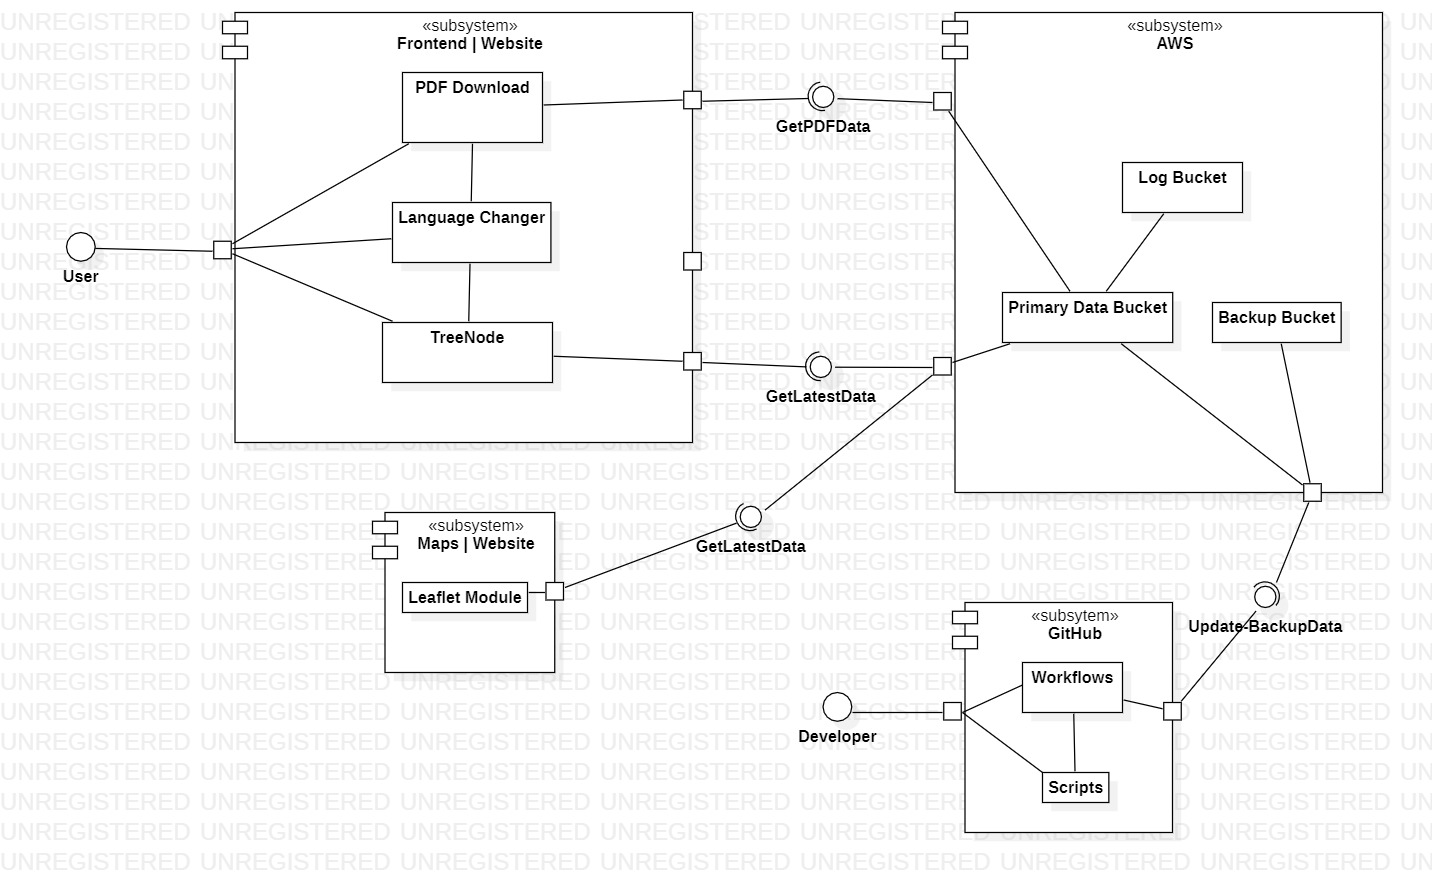
\includegraphics[width=\linewidth]{img/component-diagram.jpg}
  \caption{Component Diagram}
\end{figure}

Our system have four subsytems. Two of them subsystem is website subsytems.
\begin{itemize}
  \item The website has two different subsystems which are the frontend, the main website, and the map, providing the map feature.
  \item The map subsystem use leaflet to show the data more effectively on the map.
  \item The frontend subsystem is divided into components to handle different request from the user.
  \subitem It includes PDF component to get the PDF version of the website to use and distribute the website in offline mode. The PDF files are generated by workflows and stored in AWS.
  \subitem This subsystem also has language changer to update the language setting of the website so that user can access the website in different language to use.
  \subitem TreeNode is the main display component. It parse the data after getting the latest available data, \texttt{latest.json}, from the AWS.
  \item AWS is mainly used to \texttt{latest.json} (data), \texttt{schema.json} (schema of the \texttt{latest.json}) and PDFs.
  \item Github subsystem includes scripts and workflows. Scripts are generally written in python and used by the workflows. Workflows are responsible for checking, maintaining and updating the website in regular basis.
\end{itemize}

\subsubsection{Internal Interfaces}

\begin{figure}[H]
  \centering
  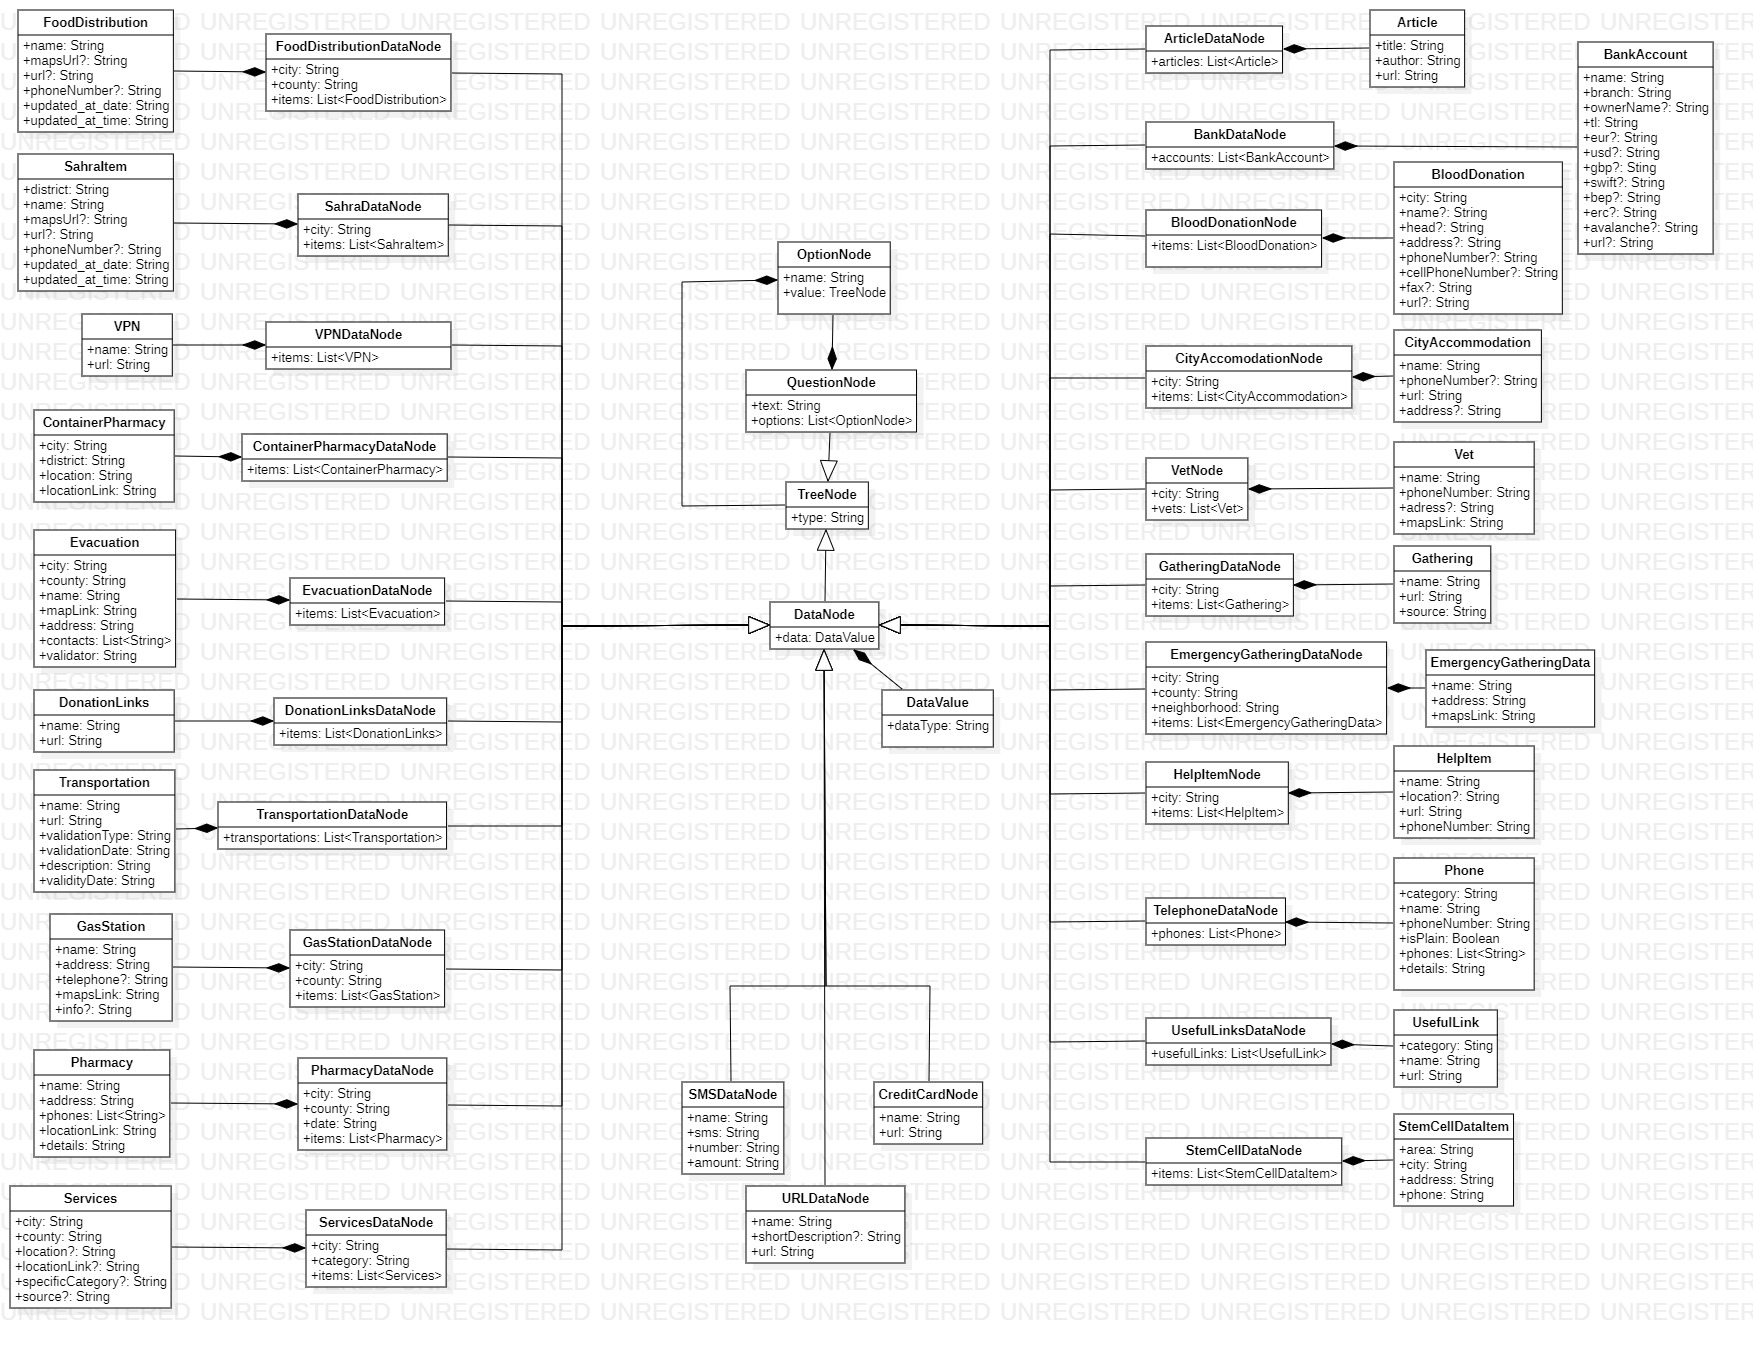
\includegraphics[width=\linewidth]{img/internal-interfaces-diagram.jpg}
  \caption{Internal Interfaces}
\end{figure}

There is no internal dynamism between interfaces. The internal interfaces are just the data interfaces to provide structured information for frontend code so that frontend code can parse the information correctly and fastly.

The main data is stored in the AWS in \texttt{latest.json} and retrieved from AWS so that the frontend code parses the data.

\subsubsection{Interaction Patterns}

\begin{figure}[H]
  \centering
  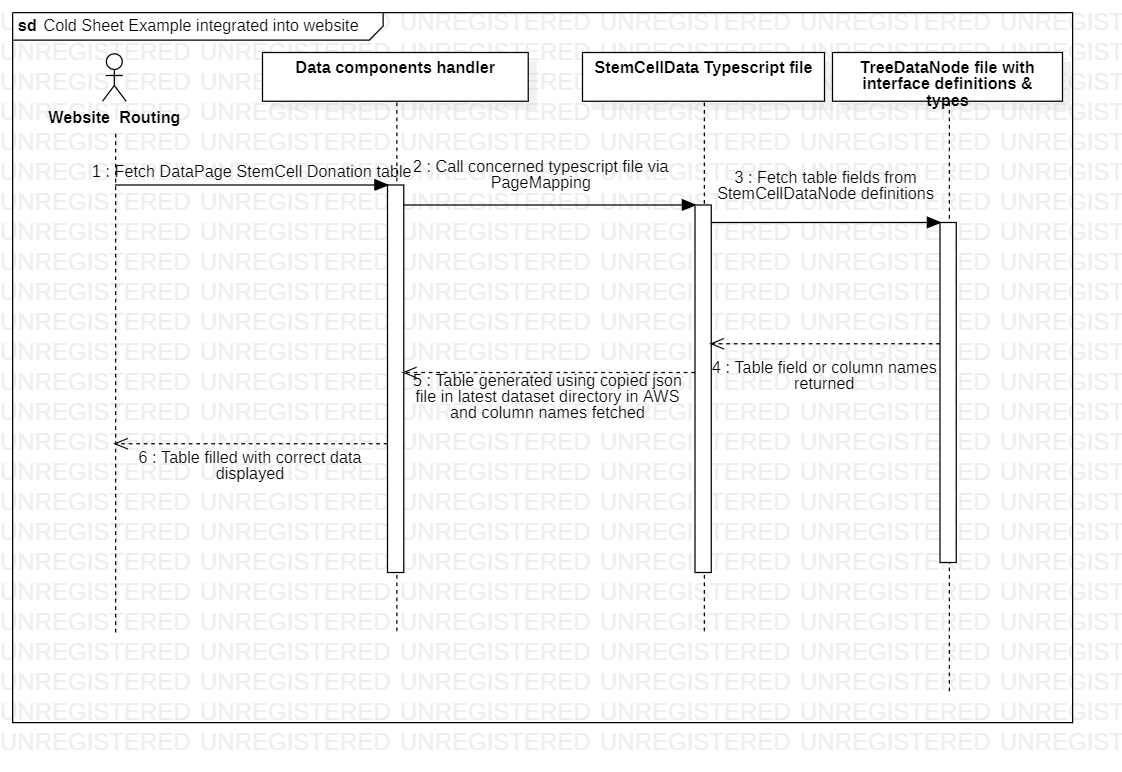
\includegraphics[width=\linewidth]{img/sequence-diagram-1.jpg}
  \caption{Sequence Diagram | Cold Sheet Example Integrated Into Website}
\end{figure}

\begin{figure}[H]
  \centering
  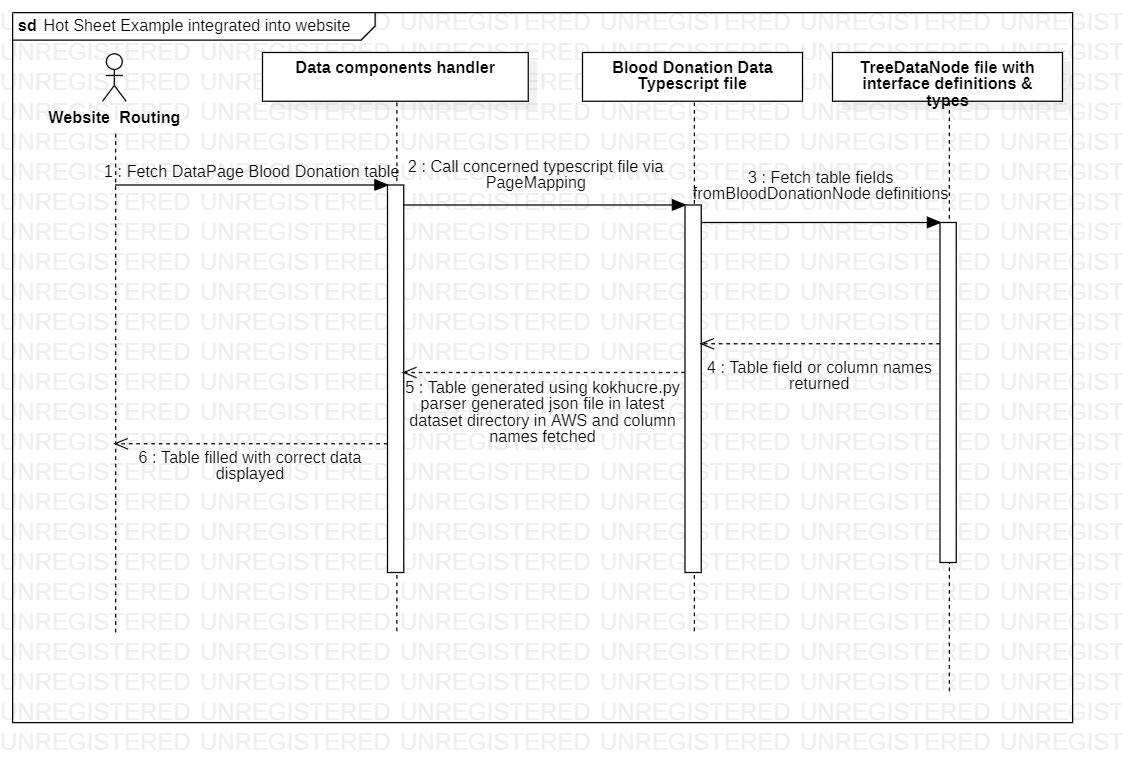
\includegraphics[width=\linewidth]{img/sequence-diagram-2.jpg}
  \caption{Sequence Diagram | Hot Sheet Example Integrated Into Website}
\end{figure}

\begin{figure}[H]
  \centering
  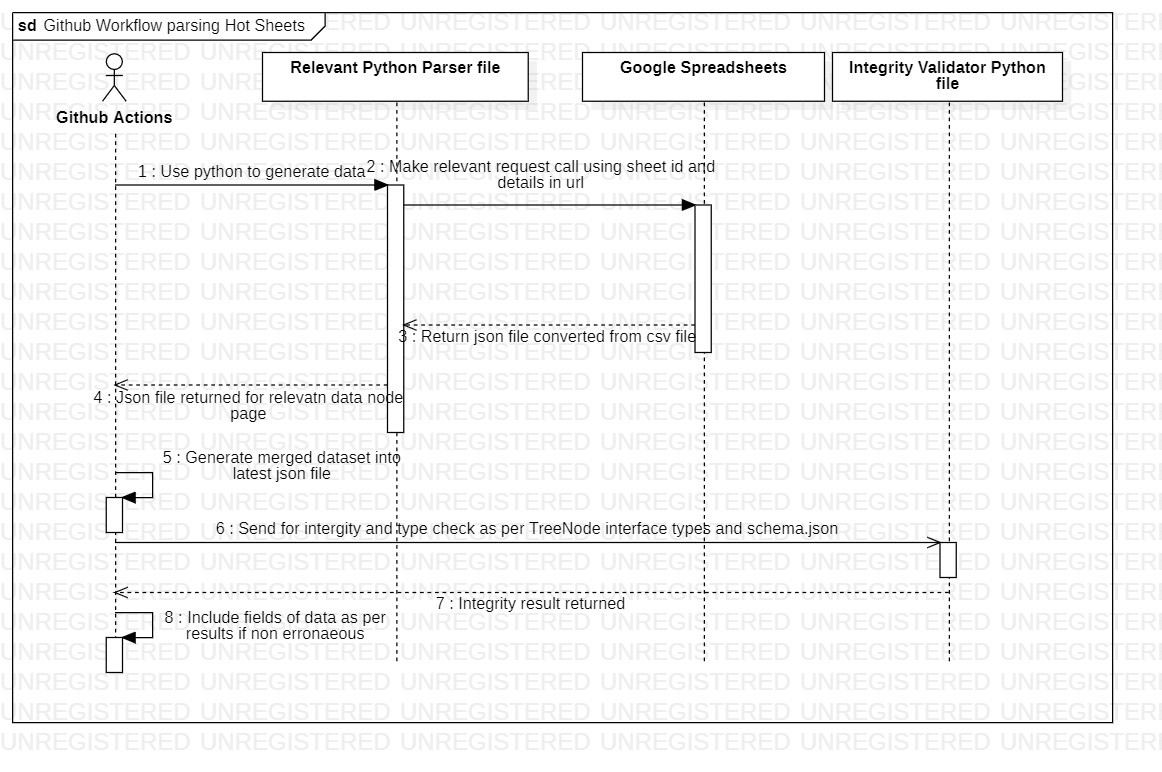
\includegraphics[width=\linewidth]{img/sequence-diagram-3.jpg}
  \caption{Sequence Diagram | GitHub Workflow Parsing Hot Sheets}
\end{figure}

\subsection{Information View}

\subsubsection{Stakeholders' Uses of This View}

\subsubsection{Database Class Diagram}

\begin{figure}[H]
  \centering
  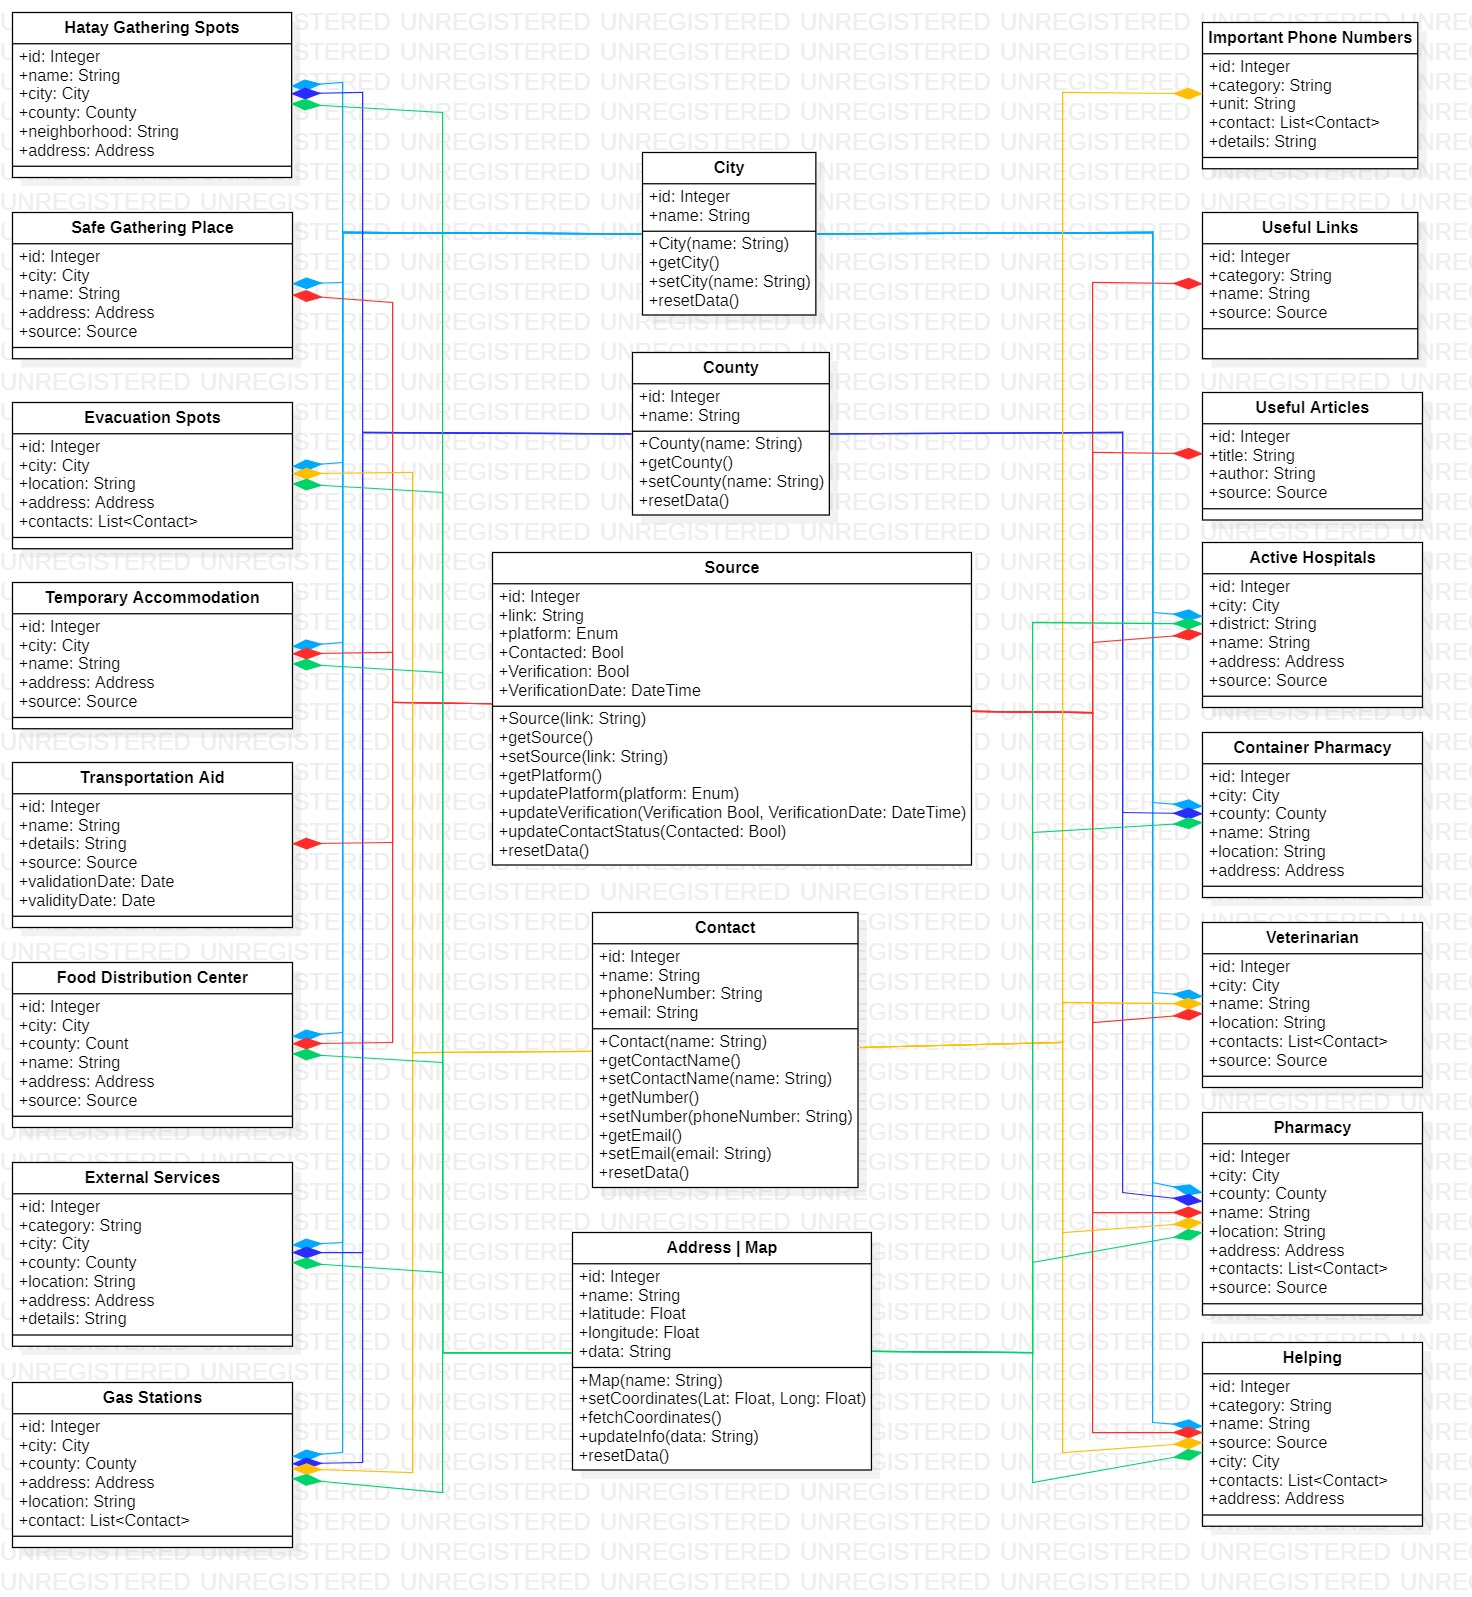
\includegraphics[width=\linewidth]{img/database-class-diagram.jpg}
  \caption{Database Class Diagram}
\end{figure}

\subsubsection{Operations on Data}

\subsection{Deployment View}

\subsubsection{Stakeholders' Uses of This View}

\subsubsection{Deployment Diagram}

\begin{figure}[H]
  \centering
  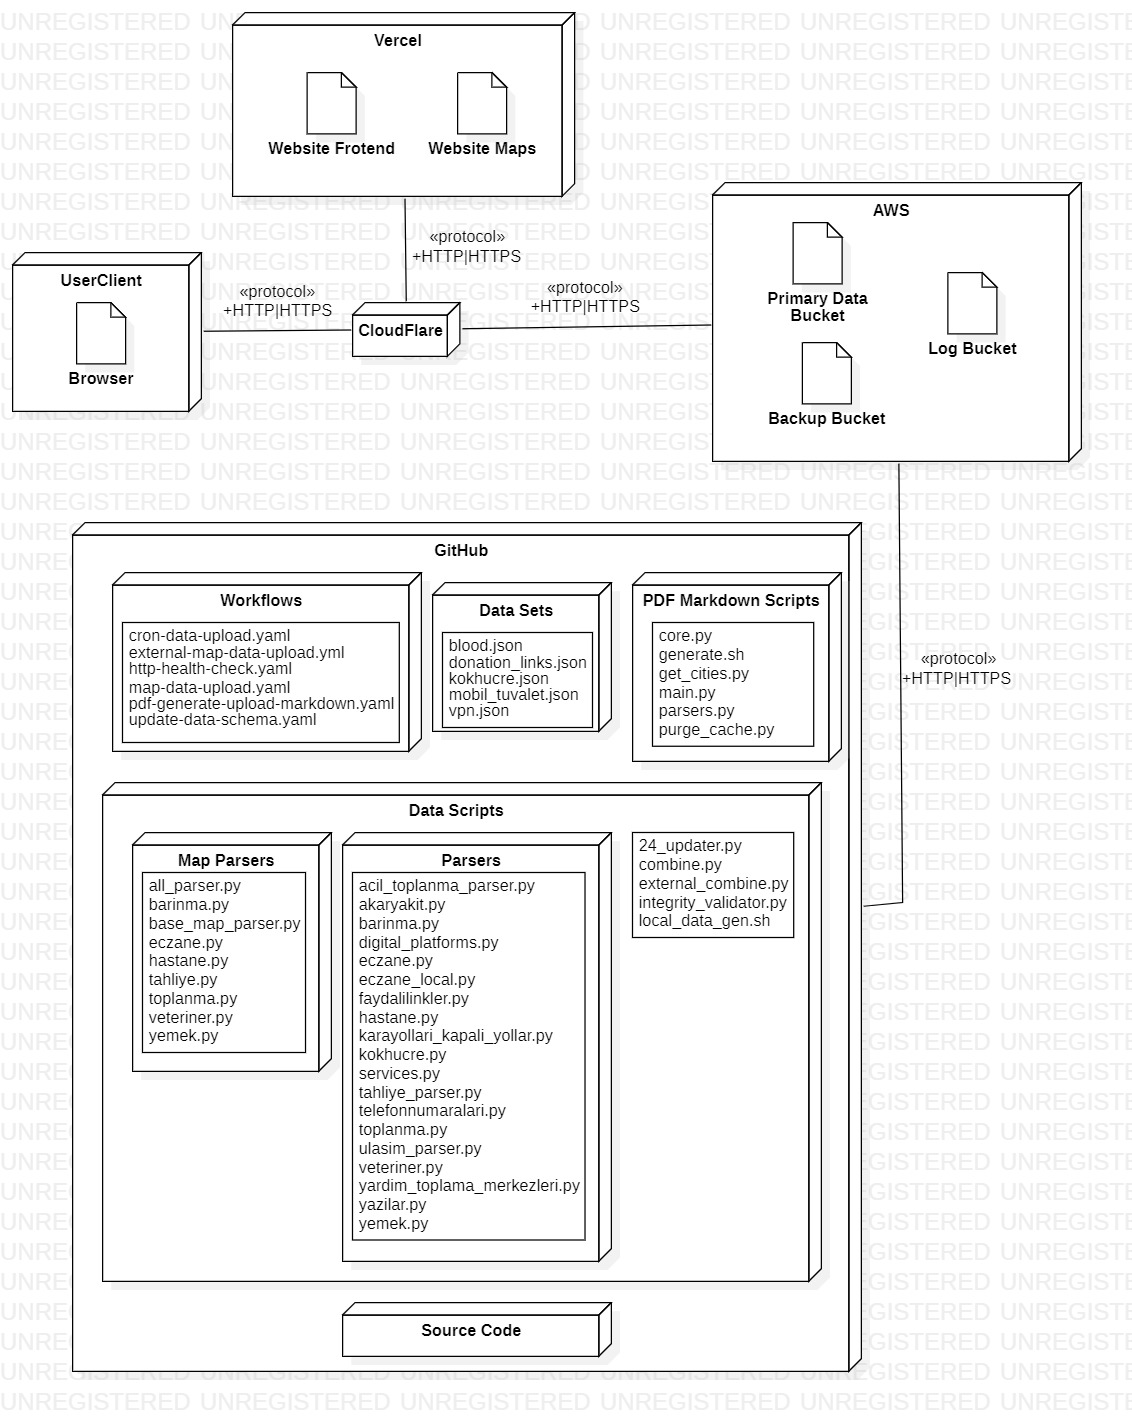
\includegraphics[width=\linewidth]{img/deployment-diagram.jpg}
  \caption{Deployment Diagram}
\end{figure}

In our deployment diagram viewpoint, we show the deployment environment of the \afetbilgi.
\begin{itemize}
  \item User should use a javascript supported browser to access the website.
  \item Requests are met by CloudFlare and CloudFlare maps the related request. CloudFlare also gives supports for general protection such as using HTTPS, TLS and DDoS protection as well as the general protection.
  \item Vercel contains the website with both frontend and maps.
  \item AWS includes the primary data which is \texttt{latest.json} and other data. It also stores the bakcups and logs.
  \item GitHub provides source code and workflows. Workflow of GitHub checks, maintains and updates the data and the website. These workflows uses scripts to get the latest and stored data data and combine them to upload to AWS. Also, PDFs are generated and upload to AWS.
  \item Google Sheets store the data updated by data collectors and validators.
\end{itemize}

\subsection{Design Rationale}
